%-------------------------------------------------------------------------------
% 请勿删除本注释
% Free Response Question 3
%
% 指引:
% 如在小问之前有通用问题描述,请放置于此
%-------------------------------------------------------------------------------
\begin{figure}[H]
\centering
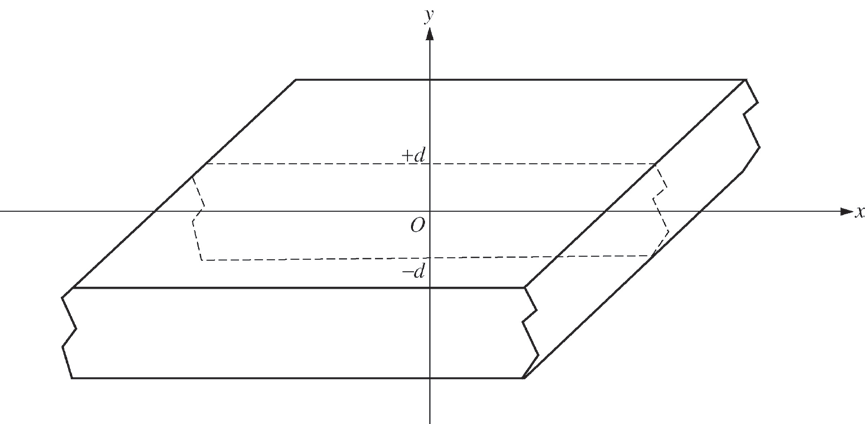
\includegraphics[scale=0.5]{images/img-016-035.png}
\end{figure}



\question
A nonconducting slab of infinite length and width and thickness $2 d$ is positioned on a coordinate system as shown above. The slab is charged, and the charge per unit volume $\rho$ is given by the expression $\rho(y)=C|y|$, where $-d \leq y \leq+d$ and $C$ is a positive constant. % 请删除并替换本行,与上一行 \question 之间不要留空行

\begin{parts}

%-------------------------------------------------------------------------------
% 请勿删除本注释
% Part (a)
%
% 指引:
% 如在小问之前有通用问题描述,请放置于此
%-------------------------------------------------------------------------------

\part
On the diagram below, do the following. % 请删除并替换本行,与上一行 \part 之间不要留空行
\begin{subparts}
\subpart Indicate with vectors the direction of the electric field at point I $(y>d)$ and point II $(0<y<d)$.
\subpart Draw a Gaussian surface that could be used to calculate the magnitude of the electric field at point I.
\end{subparts}


\begin{figure}[H]
\centering
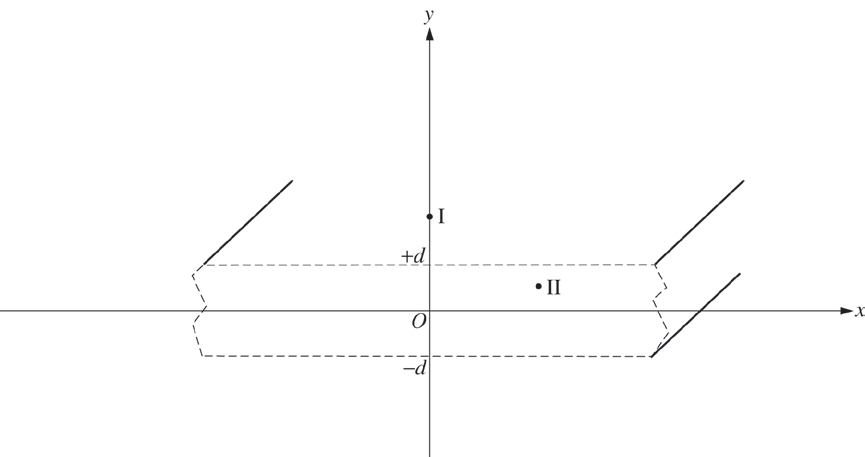
\includegraphics[scale=0.5]{images/img-016-036.png}
\end{figure}



%-------------------------------------------------------------------------------
% 请勿删除本注释
% Part (b)
%
% 指引:
% 如在小问之前有通用问题描述,请放置于此
%-------------------------------------------------------------------------------

\part
Using Gauss's law, derive expressions in terms of the given quantities and fundamental constants for the magnitude of the electric fiell $E$ at the following points. % 请删除并替换本行,与上一行 \part 之间不要留空行
\begin{subparts}
\subpart Point I $(y>d)$
\subpart Point II $(0<y<d)$
\end{subparts}

%-------------------------------------------------------------------------------
% 请勿删除本注释
% Part (c)
%
% 指引:
% 如在小问之前有通用问题描述,请放置于此
%-------------------------------------------------------------------------------

\part
Calculate the potential difference between the origin and point I. % 请删除并替换本行,与上一行 \part 之间不要留空行

\end{parts}


